\section{Simulazioni modello di Ising 2D}

Prima di iniziare lo studio computazionale del modello, è stata eseguita la necessaria determinazione dei 
parametri simulativi ottimali. In questa fase ho considerato, sia per l'algoritmo di Metropolis che per quello 
di Wolff, reticoli $N \times N$ con 

$$
N \in \left\{100,\,200,\,300,\,400,\,500\right\}
$$

alle temperature

$$
T \in \left\{1.0,\,1.5,\,2.0,\,2.5,\,3.0,\,3.5\right\}
$$

I risultati ottenuti in questa fase sono riportati in modo rissuntivo nelle seguenti figure, delle quali la 
prima è relativa al metodo di Metropolis, mentre la seconda a quello di Wolff.

\begin{figure}[H]
    \centering
    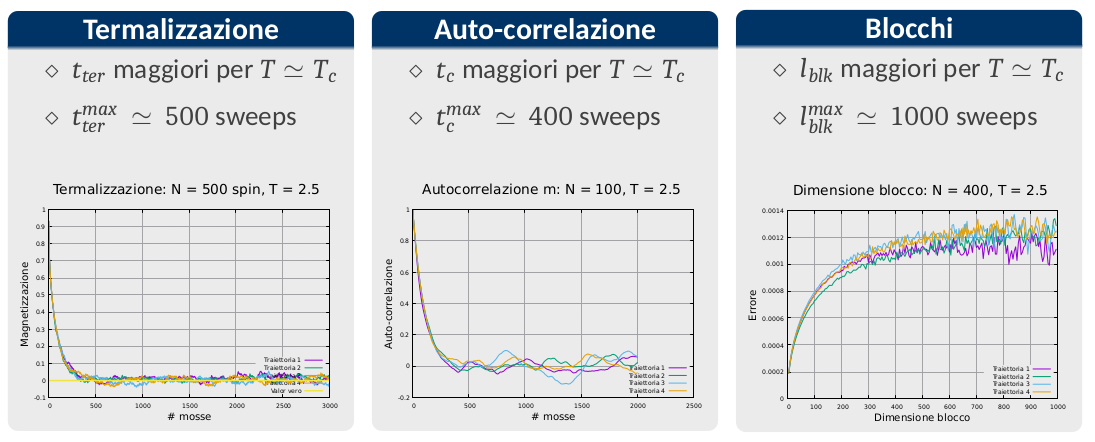
\includegraphics[width=\textwidth]{Immagini/simIsing2D/carMetro.png}
    \caption{Caratterizzazione metodo di Metropolis}
    \label{fig: car_metro}
\end{figure}

\begin{figure}[H]
    \centering
    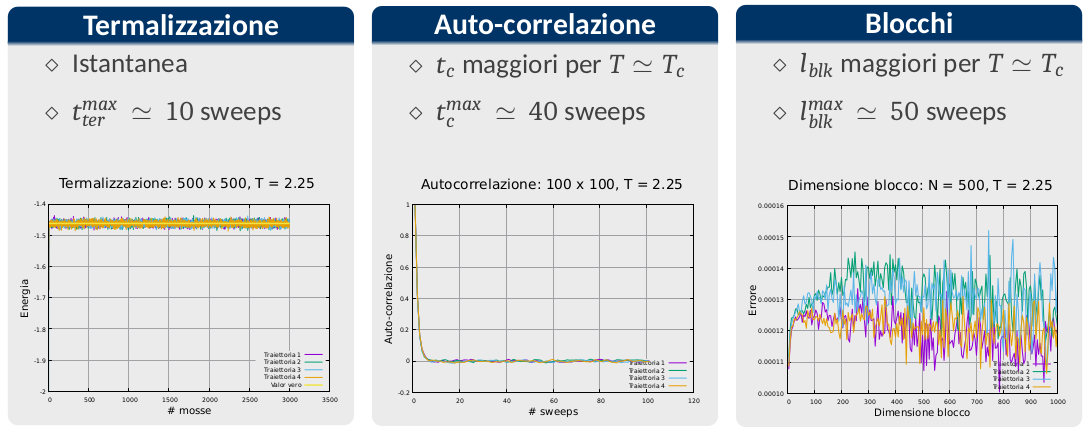
\includegraphics[width=\textwidth]{Immagini/simIsing2D/carWolff.png}
    \caption{Caratterizzazione metodo di Wolff}
    \label{fig: car_wolff}
\end{figure}





\subsection{Osservabili}

Il primo osservabile che prendiamo in considerazione è la magnetizzazione, che rende evidente la transizione di fase in quanto al di 
sotto di una certa temperatura è diversa da zero. Questo andamento è una conseguenza dell'ordine presente nel reticolo, con la spin allineati. 

\begin{figure}[H]
    \centering
    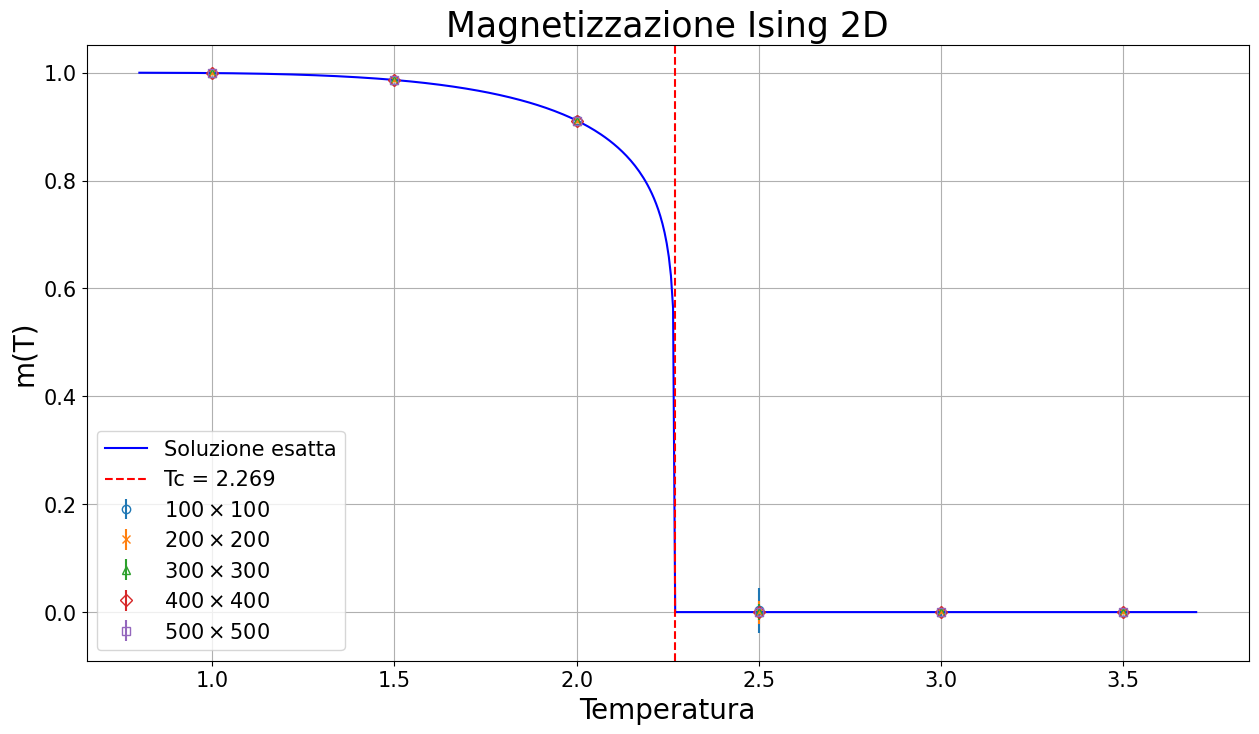
\includegraphics[width=0.9\textwidth]{Immagini/simIsing2D/magn.png}
    \caption{Magnetizzazione modello di Ising 2D: h = 0.0.}
    \label{fig: magn_Ising2D}
\end{figure}

Dato che la maggior parte degli spin sono allineati a bassa temperatura, l'energia interna assume in quella regione il suo valor minimo. 
E' possibile apprezzare $U/N$ tenda a -2, poichè i 4 "legami" che ogni spin presenta con i propri primi vicini sono condivisi con altri 
momenti magnetici. Nel momento in cui $J\,=\,1.0$, l'energia del singolo legame è unitaria e va divisa a metà sui due spin coinvolti nel 
legame.

\begin{figure}[H]
    \centering
    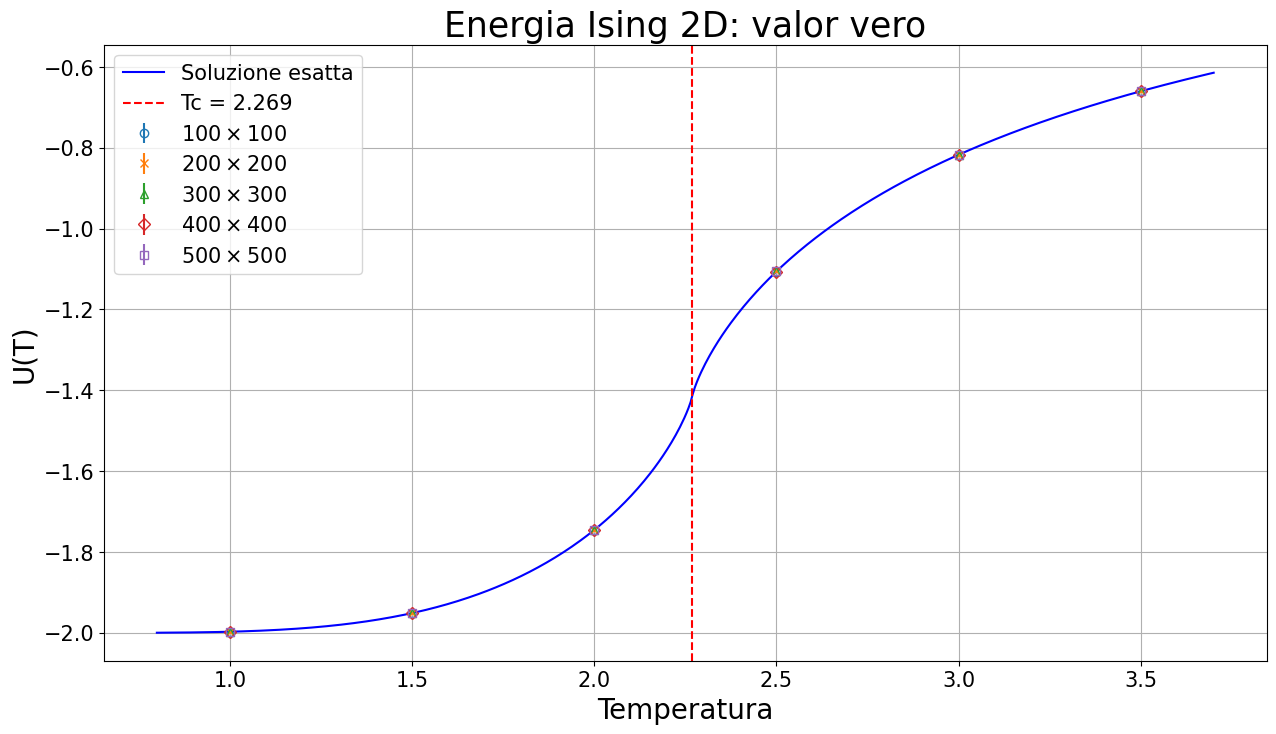
\includegraphics[width=0.9\textwidth]{Immagini/simIsing2D/ene.png}
    \caption{Energia modello di Ising 2D: h = 0.0.}
    \label{fig: ene_Ising2D}
\end{figure}





\subsection{Studio del punto critico}

L'analisi del punto critico è stata effettuata con l'algoritmo di Wolff, dato che consente la generazione di configurazioni 
scorrelate in modo molto più efficiente dell'algoritmo di Metropolis per $T \simeq T_c$. Questo studio si è concentrato inizialmente 
sulla dipendenza da $J$ della temperatura critica, che ricordiamo essere pari a

\begin{equation*}
    T_c\,=\,\frac{2J}{\log{\left(1\,+\,\sqrt{2}\right)}}
\end{equation*}

In Figura è riportata la magnetizzazione per vari valori della costante d'accoppiamento $J$ e, come si può apprezzare, 
l'algoritmo di Wolff è in grado di catturare correttamente l'andamento, anche per $T \to T_c$.

\begin{figure}[H]
    \centering
    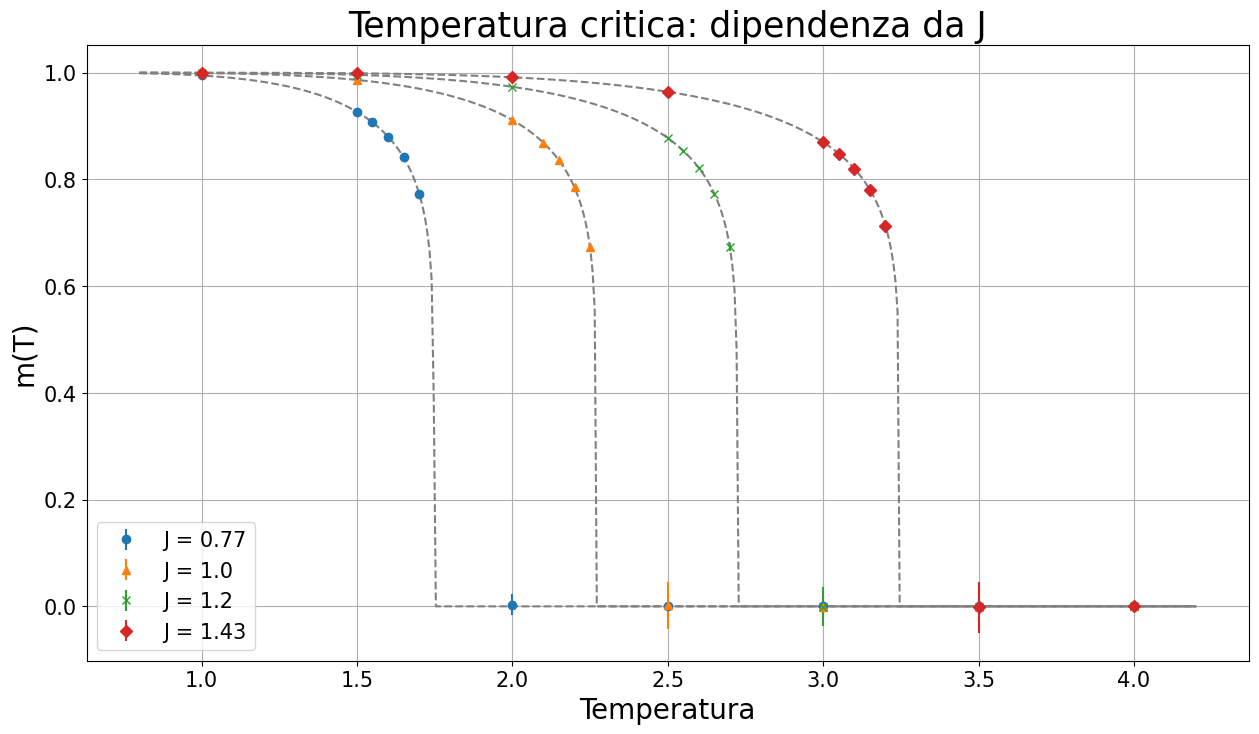
\includegraphics[width=0.9\textwidth]{Immagini/simIsing2D/dipTc.png}
    \caption{Dipendenza della temperatura critica da J.}
    \label{fig: Tc_Ising2D}
\end{figure}

Ho poi analizzato quali fossero il calore specifico e la suscettività magnetica su un certo range di temperature al variare 
della dimensione reticolare. Nelle seguenti Figure è evidente come all'aumentare di $N$, ossia il numero di spin che costituiscono 
il lato del reticolo, i risultati ottenuti rappresentano con maggior accuratezza quelli noti nel limite termodinamico.

\begin{figure}[H]
    \centering
    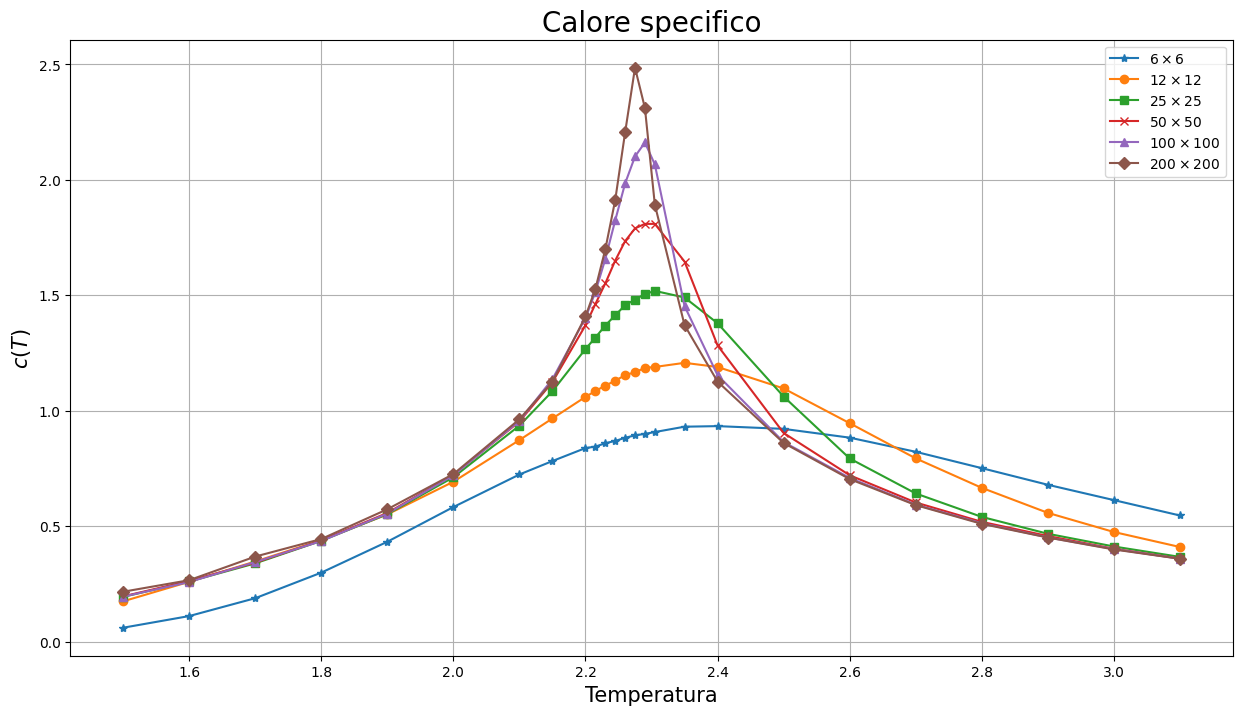
\includegraphics[width=0.9\textwidth]{Immagini/simIsing2D/cp.png}
    \caption{Calore specifico: h = 0.0.}
    \label{fig: cp_Ising2D}
\end{figure}

\begin{figure}[H]
    \centering
    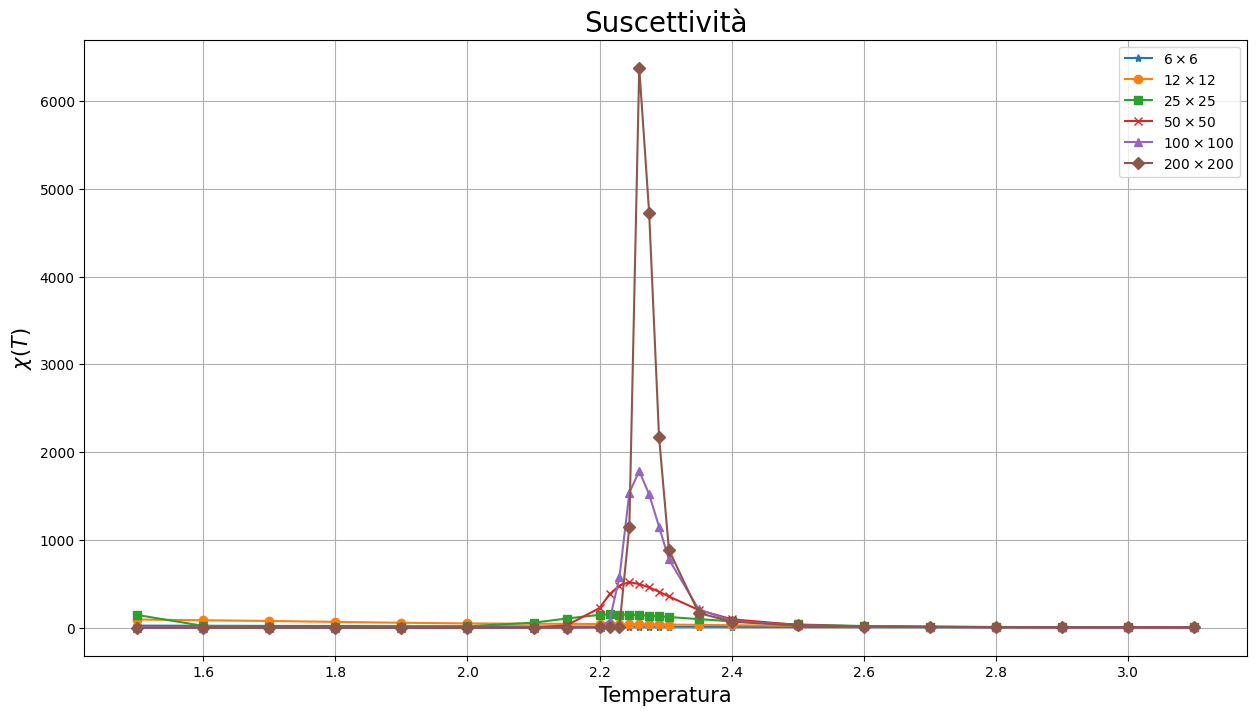
\includegraphics[width=0.9\textwidth]{Immagini/simIsing2D/chi.png}
    \caption{Suscettività: h = 0.0.}
    \label{fig: chi_Ising2D}
\end{figure}

\newpage
